\documentclass[10pt,a4paper]{article}
\usepackage[margin=2cm]{geometry}
\usepackage{graphicx}
\usepackage{amsmath,amssymb}
\usepackage{array}
\usepackage{amsthm}
\usepackage[section]{placeins}
\usepackage{setspace}
\usepackage{enumerate}
\usepackage{fullpage}
%\usepackage{subfigure}
\usepackage{caption}
\usepackage{subfiles}
% \usepackage{subcaption}
\usepackage{tikz}
\usepackage{algorithm}
\usepackage{algorithmic}
\usepackage{listings}
\usepackage{color}
\usepackage[caption=false]{subfig}
\usepackage{xcolor, colortbl}


% \definecolor{green}{rgb}{0.1,0.1,0.1}

\parindent 0pt
\everymath{\displaystyle}
\title{CSA 250 : Deep Learning Project III \\ Report}
\author{Magare Aadesh Gajanan (15605)}
\date{\today}

\setlength{\parskip}{0.5em}

\newtheorem{theorem}{Theorem}
\newtheorem{definition}{Definition}
\newtheorem{proposition}{Proposition}
\newtheorem{corollary}{Corollary}
\newtheorem{lemma}{Lemma}

\DeclareMathOperator*{\argmin}{arg\,min}
\DeclareMathOperator{\scriptL}{\mathcal{L}}
\newcommand{\olambda}{\overline{\lambda}}


\begin{document}

\maketitle
\section{Task}

The project is to implement a deep network for the task of Natural Language Inference. Given two sentences, we will predict if the sentence pair constitutes entailment/contradiction/neutral. We'll build a simple Logistic regression classifier using TF-IDF features and a deep learning model specific for text like LSTM.


\section{Dataset}
We would use one of the standard datasets for this task called Stanford Natural Language Inference (SNLI). We would primarily use the files snli\_1.0\_train.jsonl for training the model and snli\_1.0\_test.jsonl for evaluating the performance of the model. In each of these files the relevant fields to be considered are gold\_label, sentence1 and sentence2. 

Where sentence1 is the first sentence of the pair. This is also called premise. sentence2 is the second sentence in the pair. This is also called hypothesis and gold\_label represents the target label.


\section{Approach}
I tried two different architectures for the task i.e. simple logistic regression classifier using TF-IDF features and deep learning based model like LSTM. For both the approaches I'll present how I arrived on final architecture, justify different architectural choices and hyper parameter tuning strategy.

\subsection{Logistic Regression Classifier using TF-IDF Features}

The training data consists of two sentences and a corresponding label. We first take the TF-IDF features for both the sentences of a training example and concatenate them. The resultant vector is passed through a simple logistic regression classifier to predict the label. The simple baseline model gives an accuracy of \textbf{55.09 \%} on the validation set. Figure \ref{lrloss} shows the training and validation loss during the training process.

\begin{figure}[h!]
\begin{center}
	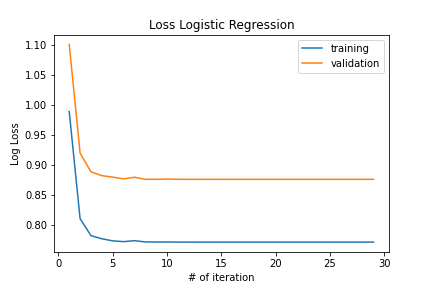
\includegraphics[width=0.85\linewidth]{loss_lr.png}
	\caption{Logistic Regression Loss}
	\label{lrloss}
\end{center}
\end{figure}

	Next we'll explore some architectural changes in the model to achieve better performance. We'll pre-process the input to better differentiate between the premise and hypothesis sentences. Each word from premise is appended with token 's1\_' while each word from hypothesis is appended with token 's2\_'. Following the pre-processing the same model gives a validation accuracy of \textbf{64.61\%}. 

Then We'll try removing the stop words which is standard practice in NLP, however it gives no improvement in model performance but further decreases the accuracy by 0.5\%. 

Next we'll employ stemming by using NLTK package, stemming helps by only a slight amount with model performance and the resultant model accuracy is slightly higher (0.07\%). However lemmetization does not help in this case and further reduces model accuracy.
 
\textbf{Hyper-Parameters Tuning} After choosing the best model so far i.e. we'll tune the remaining hyper-parameters.
\begin{enumerate}
\item \textbf{ngram\_range:} We'll try out different commonly used values of ngram for CountVectorizer i.e. (1, 1),  (1, 2), (2, 2). 
\item \textbf{stop\_words} whether to remove stop words or not
\item \textbf{TF\_IDF} Several hyper parameters associated with TF-IDF such as whether to use IDF or not, smooth IDF or not and the penalty to be used l1, l2 or None.
\item \textbf{Solver} What solver to be used in logistic regression classifier, we'll try several values such as 'newton-cg', 'sag', 'saga', 'lbfgs' along with the choice of regularization for each one of them.
\end{enumerate}

Grid Search is used for searching optimal hyper parameters. The resultant model gives validation accuracy of \textbf{67.42\%}. The optimal hyper parameters for the model are ngram\_range of (1, 2), removing English stop words, using IDF and the solver of type 'saga'.

\begin{table}[h!]
\centering
\begin{tabular}{|c| c|} 
 \hline
 Model & Validation Accuracy (\%) \\
 \hline\hline
 Baseline & 55.09 \\ 
 \hline
 preprocessing with s\_1 and s\_2 tokens & 64.61 \\ 
 \hline
 stemming & 64.68 \\ 
 \hline
 Best model + tuned Hyper parameters & 67.42 \\ 
 \hline
\end{tabular}
\caption{Summary of different architectural choices (Logistic Regresion)}
\label{table:2}
\end{table}

Finally we take the best performing model with tuned hyper parameters and test the performance on test set. Here it gives \textbf{accuracy of 66.41\%}. Figure \ref{mlpcm} shows the confusion matrix for test data. The dataset has several examples without label i.e. the corresponding label is '-'. Removing such examples from test set gives slightly better performance of \textbf{67.50\%}. However the confusion matrix shows the results without removing such examples. First row and column of confusion matrix shows such label less examples.
	
\begin{figure}[h!]
%\begin{center}
	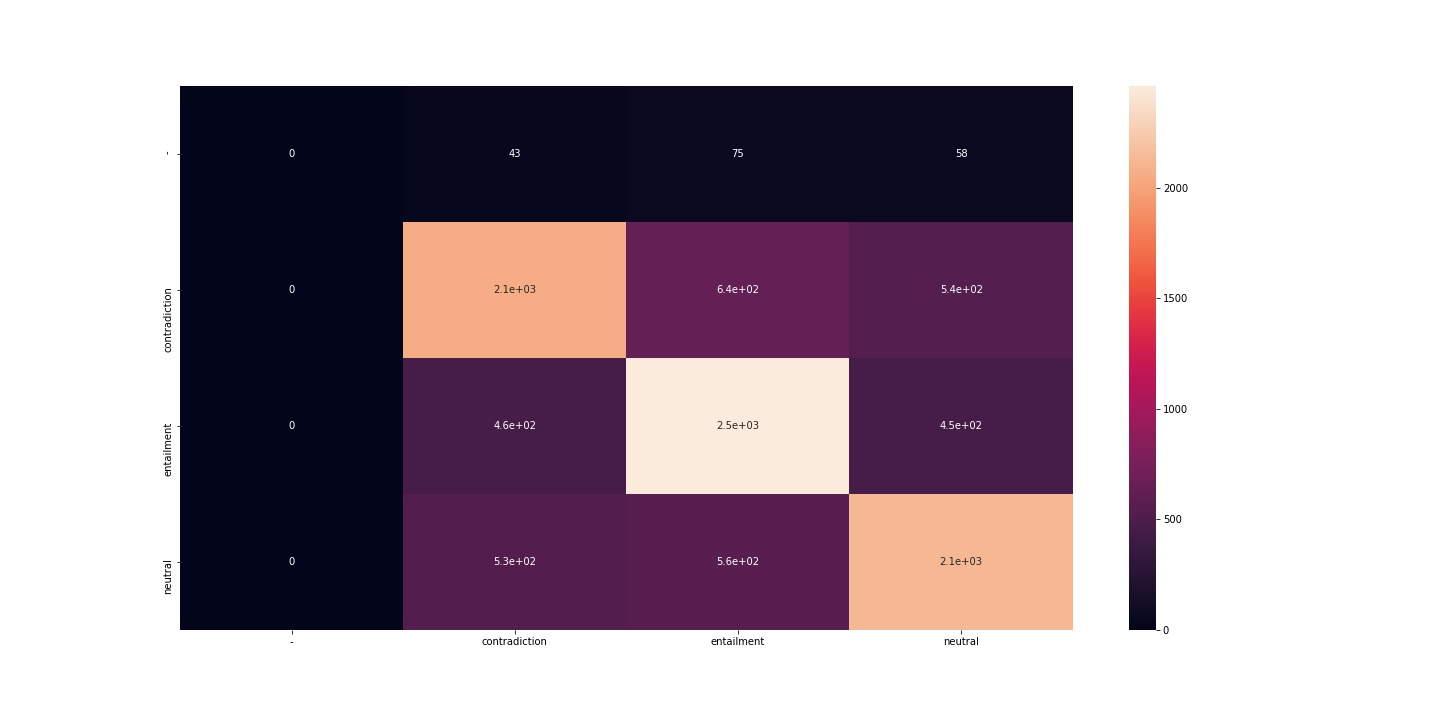
\includegraphics[width=1.3\linewidth]{cm_lr.jpg}
	\caption{Logistic Regression Confusion Matrix}
	\label{mlpcm}
%\end{center}
\end{figure}



\subsection{Deep Neural Network based approaches}

Next we'll experiment with NNs specialised for text or sequential data and will follow the same approach as logistic regression based model i.e. We'll start with simple baseline model and gradually improve it.

Starting with simple LSTM based model. We'll have an embedding layer followed by projection and LSTM layers. Final output layer is an sequential model with couple of fully connected layers. It's a multi-class classification problem thus I'll be using CrossEntropy loss. ReLu is good default choice for activation function to begin experiment, we'll see how other activation functions compare. I have used Adam optimizer with 1e-3 learning rate, which will be tuned during hyper parameter tuning phase.

	This baseline model gives accuracy of \textbf{77.16\%} on the validation set. Figure \ref{nnloss} shows the training loss and validation loss decreasing with no of epocs. Training is stopped at 10 epocs due to limitations of training resources. We'll stick to 10 epocs of training for further experiments for fair comparison. \\

\begin{figure}[h!]
\begin{center}
	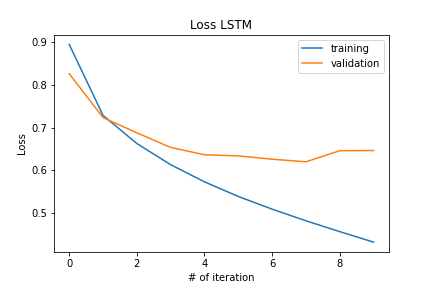
\includegraphics[width=0.85\linewidth]{loss_lstm.png}
	\caption{LSTM Loss}
	\label{nnloss}
\end{center}
\end{figure}


	Next we'll increase the capacity of network by adding additional layers and model complexity. Fully connected layers before output layer of the model can be increased for more model capacity. We'll vary the fully connected layers from 1 to 3 before the output layer. \\
	
	Further the LSTM layer used can be enhanced with stacked LSTM making it 2 or 3 layer LSTM. Apart from this we can use BiLSTM in place of simple LSTM layer. Apart from this we'll experiment with the use of pre-trained word embeddings like Glove. Apart from LSTM, the core model can be changed to GRU or a TransformerEncoder. Due to lack of training resources we're restricting the training to 10 epocs thus a very large model like transformer is not able to show expected performance and the performance is less than that of LSTM.
	
	We'll choose the best performing architecture giving validation accuracy of \textbf{77.47\%} out of this for further experiments involving hyper parameter tuning.
		
\textbf{Regularization:} Following forms of regularization were tried, it was also observed that combining multiple forms of regularization does not help to improve performance.\\

\begin{enumerate}

\item \textbf{L2 penalty} L2 regularization is a widely used regularization method for linear models. It's rarely used in DNN models and here the resultant model shows no performance gain with it but further reduces accuracy by about 1\%. 

\item \textbf{Dropout} It's the de-facto regularization method for many tasks and shown to prevent over-fitting in wide variety of network architectures. Here the resultant model shows an increase of 0.6\% to 0.8\% of increase in accuracy.

\end{enumerate}

Next we try different activation functions i.e. Sigmoid, Tanh, ReLU. as expected ReLU performs the best from the alternatives. Sigmoid gives 2.6\% reduction in accuracy where as using tanh drastically hinders the model performance.

\textbf{Hyper-Parameters tuning} After choosing the best model so far i.e. Bidirectional LSTM model with just 1 layer and dropout regularization along with ReLU activation function, we'll tune the remaining hyper-parameters.

\begin{enumerate}
\item \textbf{Learning rate} is probably the most important hyper parameter, I've started with good default of 1e-3 and used "ReduceLROnPlateau" learning rate scheduler in PyTorch. It gradually decreases the learning rate upon reaching a plateau. Here for the scheduler to work better, the model is trained for 15 epocs. Resultant model gives accuracy of 78.30\% on validation set.

\item \textbf{Batch Size} affects both the training speed and the accuracy of resultant model, I have tried several values for batch size and 512 gives the best results.

\end{enumerate}

After all hyper-parameter tuning and using learning rate scheduler we get a validation accuracy of \textbf{78.30\%.}. Table \ref{table:2} gives the summary of overall experiments.

\begin{table}[h!]
\centering
\begin{tabular}{|c| c|} 
 \hline
 Model & Validation Accuracy (\%) \\
 \hline\hline
 Baseline (1 conv layer) & 91.03 \\ 
 \hline
LSTM Based & 77.47 \\ 
 \hline
 GRU Based & 75.74 \\ 
 \hline
TransformerEncoder Based & 33.80 \\ 
 \hline
Stacked LSTM Based  & 76.86 \\ 
 \hline
LSTM Based with tuned HP & \textbf{78.30} \\ 
 \hline
\end{tabular}
\caption{Summary of different architectural choices (NN) }
\label{table:2}
\end{table}

Finally we take the best performing model and test the performance on actual test set. Here it gives \textbf{accuracy of 77.41\%}. Figure \ref{nncm} shows the confusion matrix for test data. 

\begin{figure}[h!]
%\begin{center}
	\includegraphics[width=1.3\linewidth]{cm_NN.png}
	\caption{LSTM Confusion Matrix}
	\label{nncm}
%\end{center}
\end{figure}


Table \ref{table:3} shows the performance of both logistic regression based model and LSTM based model on the actual test dataset. LSTM model clearly performs better than logistic regression model with \textbf{11\%} better accuracy, which clearly shows it's superiority for textual data and preserving long term dependency.

\begin{table}[h!]
\centering
\begin{tabular}{|c| c|} 
 \hline
 Model & Test Set Accuracy (\%) \\
 \hline\hline
Logistic Regression Based & 66.41 \\ 
 \hline
LSTM Based & 77.41 \\ 
 \hline

\end{tabular}
\caption{Result on test dataset }
\label{table:3}
\end{table}


\bibliographystyle{IEEEtran}
\bibliography{references.bib}
\end{document}
